%TODO : Réordonner
% mettre en reserve les moulins a vent et l'exo 5 2010 et les caméléons

\subsubsection{Introduction}
Le concept d'invariant n'est que rarement utilisé dans des problèmes "statiques", où la situation est immuable. Par contre, certains problèmes sont "dynamiques" : il s'agit de passer d'une configuration initiale à une configuration finale, en respectant certaines règles sur les transformations effectuées. Dans ce cas, un invariant est une quantité que l'on peut associer à chaque état du problème et qui ne varie jamais lorsqu'on applique une des transformations autorisées. Si les quantités associées aux configurations initiale et finale sont différentes, on a alors démontré l'impossibilité de passer de l'une à l'autre.\\

\begin{exo}
On se donne le tableau rempli de signes suivant :
\begin{align*}
& ++-+\\
& --++\\
&++++\\
& +-+-
\end{align*}
Un coup consiste à choisir une ligne ou une colonne et changer les signes présents dedans. Est-il possible d'arriver en un nombre fini de coups à un tableau rempli de signes $+$?
\end{exo}

\begin{sol}
La parité du nombre de signes $-$ est un invariant. Ce nombre est impair dans la position initiale, on ne peut donc pas atteindre une position qui aurait $0$ signe $-$.
\end{sol}


De même, il peut arriver qu'une quantité associée à chaque configuration croisse (resp. décroisse) à chaque transformation appliquée. On parle alors de monovariant. Il est bien entendu impossible de parvenir à une configuration où ce monovariant est plus petit (resp. plus grand) que la configuration initiale. De plus, si le monovariant est majoré et augmente d'au moins une certaine quantité non nulle fixée à chaque transformation, on peut conclure que le processus d'application des transformations prend forcément fin.\\

\begin{exo}
Sur un tableau, on écrit $n$ fois le chiffre $1$. Une opération consiste à choisir deux nombres $a$ et $b$ écrits au tableau, à les effacer et à écrire $\frac{a+b}{4}$ à la place. Montrer que le nombre écrit au tableau au bout de $n-1$ étapes est supérieur ou égal à $\frac1{n}$.
\end{exo}

\begin{sol}
On peut remarquer que $\frac1{a}+\frac1{b}\geq \frac{4}{a+b}$ (il suffit de tout mettre au même dénominateur et de faire apparaîte $(a-b)^2\geq0$). Dès lors, la somme des inverses des nombres écrits au tableau est décroissante lorsqu'on applique une transformation. Elle vaut $n$ dans la position initiale, donc dans la position finale elle est inférieure à $n$ : le dernier nombre est dès lors supérieur à $\frac1{n}$.
\end{sol}

\begin{exo}
Il y a $2021$ mésanges qui nichent sur $120$ arbres. Essayant de les déloger, un chasseur maladroit leur tire dessus. A chaque fois, il manque sa cible mais effraie une mésange qui quitte alors son arbre et se réfugie sur un arbre avec au moins autant de mésanges que son arbre de départ (elle se compte sur ce dernier). Montrer qu'après un certain nombre fini de tirs, toutes les mésanges seront sur le même arbre.
\end{exo}

\begin{sol}
L'ordre lexicographique entre listes dont les éléments font partie d'un ensemble totalement ordonné est défini comme suit. Une liste est toujours plus petite qu'une liste plus longue. Si les listes ont la même longueur, on regarde le premier élément de chaque liste. S'ils sont différents, la liste ayant le plus petit premier élément est la plus petite. Si ils sont égaux, on passe au deuxième élément, et ainsi de suite. Par exemple, si on considère les mots comme des listes de lettres, l'ordre lexicographique entre listes de même longueur correspond à l'ordre du dictionnaire.\\
Représentons une configuration par la liste du nombre de mésanges sur chaque arbre, triée par ordre croissant. Quand le chasseur tire, un des nombres de la liste diminue de $1$ et un nombre situé plus loin dans la liste augmente de $1$. Dès lors, la nouvelle liste est strictement plus petite par ordre lexicographique que la première. Comme il n'y a qu'un nombre fini de listes de $120$ éléments naturels dont la somme fait $2021$, on finira par atteindre en un nombre fini d'étapes la plus petite, qui correspond à avoir toutes les mésanges sur un même arbre.
\end{sol}


Parfois, on peut montrer l'impossibilité d'une construction en coloriant la surface sur laquelle elle doit se dérouler. On peut voir le coloriage comme une façon de créer un invariant.\\

\begin{exo}
Sur une grille $2022\times2022$, on peut bouger un jeton d'une case vers une autre si ces deux cases ont un côté commun. Est-il possible, en partant avec le jeton dans le coin inférieur gauche, d'amener le jeton dans le coin supérieur droit en passant une et une seule fois par toutes les cases?
\end{exo}

\begin{sol}
En coloriant la grille comme un damier, on voit qu'un déplacement vers une case ayant un côté commun change la couleur de la case sur laquelle on se trouve. De plus, les cases de départ et d'arrivée sont de la même couleur, il faut donc avoir réalisé un nombre pair de mouvements pour passer de l'une à l'autre. Mais si l'on visite toutes les cases de la grille, on aura fait $2018^2-1$ déplacements, ce qui est impair, d'où une impossibilité.
\end{sol}

\subsubsection{Exercices}

\begin{exo}
Les nombres entiers de $1$ à $2018$ sont écrits au tableau. Une opération consiste à en choisir deux, les effacer et réécrire sur le tableau la valeur absolue de leur différence. Montrer que le dernier nombre écrit au tableau est impair.
\end{exo}

\begin{exo}
On a $2018$ piles de jetons. Sur la $i$-ème pile, il y a $p_i$ jetons, où $p_i$ est le $i$-ème nombre premier. On s'autorise :
\begin{itemize}
\item
à séparer une pile en deux autres et ajouter un jeton à l'une des deux piles ainsi créées.
\item
à fusionner deux piles et ajouter un jeton à la pile créée.
\end{itemize}
Peut-on aboutir à la situation avec $2018$ piles de $2018$ jetons chacune?
\end{exo}

\begin{exo}
Dans l'espace, on part de l'ensemble de $7$ sommets d'un cube. On s'autorise à remplacer un point par son symétrique par rapport à un autre point. Peut-on atteindre le huitième sommet de cette façon?
\end{exo}

\begin{exo}
On écrit un signe $+$ ou $-$ sur chaque case d'un tableau $8\times8$. Une opération consiste à choisir un carré $3\times3$ ou $4\times4$ et inverser les signes présents dedans. Peut-on toujours atteindre un tableau rempli de $+$?
\end{exo}

\begin{exo}
Un sol rectangulaire est pavé par des rectangles $4\times1$ et $2\times2$. Si l'on casse un des carreaux, peut-on le remplacer par un carreau de l'autre type et repaver le sol?
\end{exo}

\begin{exo}
$n$ points du plan sont coloriés en rouge, $n$ autres le sont en bleu. Ces $2n$ points ne sont pas $3$ à $3$ alignés. Est-il possible de tracer $n$ segments reliant un point rouge à un point bleu, chaque point étant utilisé une seule fois, de manière à ce que deux segments ne s'intersectent jamais?
\end{exo}

\begin{exo}
Est-il possible de paver (sur plusieurs couches) un rectangle $5\times 7$ par des trominos en L de manière à ce que chaque case soit recouverte par le même nombre de trominos?
\end{exo}

\begin{exo}
Sur une ligne, on écrit $2018$ entiers naturels. Ensuite, pour chaque ligne, on écrit en-dessous de chaque entier le nombre de fois qu'il apparaît dans la ligne, créant ainsi une nouvelle ligne en-dessous de la première, sur laquelle on réapplique le processus. Montrer qu'au bout d'un certain temps toutes les lignes qu'on écrit deviennent identiques.
\end{exo}

\begin{exo}
De combien de manières peut-on paver un damier $10\times10$ par des tétraminos en T?
\end{exo}

\begin{exo}
$2009$ cartes, ayant chacune un côté bleu et un côté jaune, sont alignées côté bleu sur une table. Deux personnes situées du même côté de la table jouent alors en alternance. Un coup consiste à choisir un bloc de 50 cartes dont la carte la plus à gauche est bleue et à retourner toutes les cartes du bloc. La personne qui ne peut plus jouer perd. Le jeu se termine-t-il forcément? Si oui, qui a une stratégie gagnante?
\end{exo}

%TODO : Croatie
\begin{exo}
Chaque case d'un damier de taille $n\times n$ contient une lampe. Au début, deux lampes situées dans deux coins opposées sont allumées, et les autres sont éteintes. Une opération consiste à choisir une ligne (rangée ou colonne) du damier et à changer l'état de toutes les lampes dans cette ligne.\\
Avant de commencer les opérations, Alice peut choisir d'allumer individuellement autant de lampes qu'elle veut. Combien de lampes doit-elle allumer au minimum pour qu'il existe une suite d'opérations après laquelle toutes les lampes sont éteintes?
\end{exo}

\begin{exo}
Sur le plan, on part du point $(1,\sqrt2)$. Quand on est en $(x,y)$, on peut se déplacer en $(x,y+2x)$, $(x,y-2x)$, $(x+2y,y)$ ou $(x-2y,y)$, mais sans revenir immédiatement au point dont on venait. Montrer qu'on ne peut revenir au point de départ.
\end{exo}

\begin{exo}
Alex et Bobette jouent sur une grille $20\times20$ où les cases sont carrées et de côté $1$. La \emph{distance} entre deux cases est la distance entre leurs centres. Ils jouent à tour de rôle de la manière suivante : Alex met une pierre rouge sur une case, de manière à ce que la distance entre deux cases portant des pierres rouges ne soit jamais $\sqrt5$, puis Bobette met une pierre bleue sur la grille, sans restriction. Le jeu s'arrête quand un des deux ne sait plus poser de pierre. Trouver le plus grand $K$ tel qu'Alex peut toujours placer au moins $K$ pierres, quelles que soient les réponses de Bobette.
\end{exo}

\begin{exo}
Des entiers positifs en nombre fini sont écrits de gauche à droite sur une ligne. Lucie choisit deux nombres voisins $x$ et $y$ tels que $x$ est à gauche de $y$ et $x>y$ et remplace la paire $(x,y)$ par $(x-1,x)$ ou $(y+1,x)$ au choix, puis recommence tant que possible. Montrer qu'elle ne peut continuer indéfiniment.
\end{exo}

\begin{exo}
Les participants du stage Animath s'appellent $C_1,\ldots,C_n$ et font la file devant le restaurant selon les règles suivantes :
\begin{itemize}
\item
Les animatheurs choisissent l'ordre initial des participants.
\item
A chaque étape, les animatheurs choisissent un entier $i$ avec $1\leq i\leq n$. Si le participant $C_i$ a au moins $i$ personnes devant lui dans la queue, il paie 1 euro aux animatheurs et avance de $i$ places. Sinon, le restaurant ouvre et le processus se termine.
\end{itemize}
Montrer que le processus se termine forcément et déterminer la quantité maximale d'argent que les animatheurs peuvent extorquer aux participants.
\end{exo}

\begin{exo}
Il y a une lampe sur chaque case d'une grille $5\times5$. Lorsqu'on allume ou éteint une lampe, ses voisines par un côté changent également d'état. Initialement, toutes les lampes sont éteintes. Martin arrive et active certains interrupteurs. Au final, une seule lampe est allumée. Quelles sont ses positions possibles?
\end{exo}

\subsubsection{Solutions}

\begin{sol}
A chaque étape, la somme des nombres impliqués dans la transformation passe de $a+b$ à $a-b$ ou $b-a$, elle est donc modifiée d'une quantité paire ($2b$ ou $2a$ respectivement). La parité de la somme des nombres écrits au tableau est donc un invariant. Dans la situation initiale, elle vaut $\frac{2018\cdot 2019}2=1009\cdot 2019$ qui est impair. Après $2017$ étapes, il ne reste plus qu'un nombre au tableau, qui doit être impair.
\end{sol}

\begin{sol}
En traitant les diverses possibilités de mouvement, on remarque que la parité du nombre de piles de hauteur paire reste inchangée. Comme ce nombre est impair dans la position initiale et pair dans la position à atteindre, il est impossible d'aboutir à cette dernière.
\end{sol}

\begin{sol}
Plaçons-nous dans un repère orthonormé où les sept points du cube ont pour coordonnées $(0,0,0),(0,0,1),(0,1,0),(1,0,0),(0,1,1),(1,0,1)$ et $(1,1,0)$. Le symétrique du point $(a,b,c)$ par rapport au point $(a',b',c')$ est le point $(2a'-a,2b'-b,2c'-c)$. En particulier, la parité des coordonnées est invariante par ces symétries. On ne peut donc atteindre le point $(1,1,1)$ puisque ses trois coordonnées sont impaires.
\end{sol}

\begin{sol}
Ici, la parité du nombre de signes $-$ n'est plus un invariant, mais on peut remarquer que la parité du nombre de signes $-$ en dehors des troisième et sixième colonnes en est un. La configuration demandée n'est donc pas toujours atteignable.
\end{sol}

\begin{sol}
On colorie le sol en répétant le motif
\begin{align*}
&ABAB\ldots\\
&CDCD\ldots\\
&ABAB\ldots\\
&CDCD\ldots\\
&\vdots\quad\vdots\quad\vdots
\end{align*}
Un rectangle $2\times2$ couvre une case de chaque couleur, tandis qu'un rectangle $1\times4$ en couvre $2$ d'une couleur et $2$ d'une autre. Ils ne sont donc pas interchangeables. (La parité du nombre de cases de chaque couleur pavées doit rester constante, or elle ne le sera pas ici).
\end{sol}

\begin{sol}
Si deux segments $AB$ et $CD$, avec $A$ et $C$ rouges, ont une intersection, alors les segments $AD$ et $CB$ n'en ont pas et la somme de leurs longueurs est plus petite que celle des longueurs de $AB$ et $CD$. Il n'y a que $n!$ manières d'apparier les points. En prenant celle où la somme des longueurs des segments est la plus petite, et vu la remarque précédente, il n'y aura aucune intersection. Cet exercice illustre le lien entre les méthodes par monovariant et les méthodes à base d'extremum.
\end{sol}

\begin{sol}
Si on réutilise le coloriage de l'exercice $19$ en plaçant un $A$ dans le coin en haut à gauche, on a $12$ $A$ sur le rectangle, mais chaque tromino ne peut recouvrir qu'un $A$. Si chaque case est recouverte $k$ fois, il faut utiliser au moins $12k$ trominos pour recouvrir tous les $A$, mais alors on a un total d'au moins $36k$ cases recouvertes et non $35k$. Il n'est donc pas possible de réaliser un tel pavage.
\end{sol}

\begin{sol}
Considérons un nombre $a$ en dehors de la première ligne. Il représente le nombre d'occurrences d'un des nombres de la ligne du dessus. Ce dernier est donc présent $a$ fois dans la ligne du dessus, et $a$ est présent au moins $a$ fois dans sa ligne. Dès lors, si on regarde une colonne, tous les nombres à l'exception du premier sont triés par ordre croissant. Comme de plus la somme des nombres d'une ligne autre que la première fait $2018$, toutes les lignes deviennent identiques au bout d'un certain temps (sinon, la somme de chaque ligne augmenterait de $1$ autant de fois que voulu, tout en restant inférieure à $2018$).
\end{sol}

\begin{sol}
Cela est impossible. En coloriant le damier comme un damier, chaque tétramino couvre $3$ cases d'une couleur et une de l'autre. En notant $n$ le nombre de tétraminos couvrant $3$ cases noires et $b$ celui de tétraminos couvrant $3$ cases blanches, on a
\begin{align*}
3n+b&=50\\
n+b&=25
\end{align*}
En soustrayant, on a $2n=25$ ce qui est impossible.
\end{sol}

\begin{sol}
Ecrivons un $1$ sur chaque face bleue et un $0$ sur chaque face jaune. A toute configuration est alors associé un nombre écrit en binaire et ayant $2009$ chiffres. Quand on fait un coup, on modifie $50$ chiffres consécutifs, dont le plus grand passe de $1$ à $0$. Le nombre associé à la position baisse donc strictement. Puisqu'il ne peut être négatif, la partie finit par s'arrêter.\\
Pour savoir qui gagne, considérons les cartes en positon $50k$ à partir de la droite, et le nombre de cartes bleues parmi celles-ci. Au début, il est de $40$, et il change de $1$ à chaque coup puisqu'exactement une de ces cartes est retournée à chaque coup. Dès lors, quand c'est au tour du second joueur, le nombre de cartes bleues parmi celles considérées est impair, donc non nul. Le second joueur a donc toujours quelque chose à jouer, et ne peut donc perdre. Puisque le jeu se finit, le second joueur gagne toujours.
\end{sol}

\begin{sol}
Notons déjà qu'il existe une solution en allumant $2n-4$ lampes : si l'on numérote les lignes et les colonnes de façon à ce que les lampes en cases $(1,1)$ et $(n,n)$ soient initialement allumées, il suffit d'allumer en plus toutes les lampes en cases $(m,1)$ ou $(n,m)$ avec $m$ entre $2$ et $n-1$, puis d'appliquer les opérations à la colonne 1 et à la ligne $n$. Montrons maintenant que $2n-4$ est la solution optimale.\par
On remarque que si l'on choisit n'importe quel rectangle de cases du damier, la parité du nombre de lampes allumées parmi les quatre coins de ce rectangle est un invariant. Dès lors, dans tout rectangle ayant pour coin une des cases $(1,1)$ ou $(n,n)$, on doit allumer au moins un autre des coins pour espérer qu'une suite d'opérations demandée existe.\par
Nous allons donc exhiber $2n-4$ rectangles dont un des coins est une des cases initialement allumées et dont les coins sont disjoints. Ainsi, on aura montré qu'il faut allumer au moins $2n-4$ cases. Les $2n-4$ rectangles annoncés sont les suivants :
\begin{itemize}
\item Les $n-2$ rectangles dont les coins sont $(1,1), (1,m), (m,1)$ et $(m,m)$, pour $m$ entre 2 et $n-1$.
\item Les $n-3$ rectangles dont les coins sont $(m,m-1), (m,n),(n,m-1)$ et $(n,n)$ pour $m$ entre 3 et $n-1$
\item Le rectangle de coins $(2,n-1), (2,n), (n,n-1)$ et $(n,n)$.
\end{itemize}
Ceci conclut.
\end{sol}

\begin{sol}
Donnons des noms aux différentes transformations : partant de $(x,y)$, appelons N le passage à $(x,y+2x)$, S pour $(x,y-2x)$, E pour $(x+2y,y)$ et O pour $(x-2y,y)$. La règle de ne pas revenir immédiatement en arrière signifie que l'on ne peut pas faire un déplacement N puis S, ou E puis O (et de même dans l'autre sens). On peut remarquer que les coordonnées du point sont toujours de la forme $(a+b\sqrt2,c+d\sqrt2)$. De plus, puisque $\sqrt2$ est irrationnel, $a$ et $c$ sont indépendants de $b$ et $d$. On peut donc montrer que partant de $(1,0)$ et suivant les mêmes règles, on ne peut revenir au point de départ, et ce sera suffisant.\\ Les mouvements E et O n'ont aucun effet au point de départ, toute séquence de coups peut donc se réécrire $a_1$N$+a_2$E$+a_3$N$+\ldots$, avec $a_i\in\Z\textbackslash\{0\}$, en notant $k$N le mouvement N répété $k$ fois, si $k>0$, et S répété $k$ fois si $k<0$, et de même pour E/O. Le mouvement $k$N correspond à passer de $(x,y)$ à $(x,y+2kx)$ tandis que $k$E correspond à passer à $(x+2ky,y)$. On peut montrer par récurrence qu'après un mouvement $k$N on a $|c|>|a|$, et $|a|>|c|$ après un mouvement $k$E. Dès lors, la distance à l'origine du point $(a,c)$ est strictement croissante (puisqu'on augmente la valeur absolue de la coordonnée la plus petite en valeur absolue, et que l'autre reste inchangée), et il est donc impossible de revenir au point de départ.
\end{sol}

\begin{sol}
Montrons que $K=100$. Alex peut toujours poser $100$ pierres : il suffit qu'il colorie la grille en damier et qu'il joue toujours sur une case blanche. En effet, deux cases blanches ne sont jamais à distance $\sqrt5$ l'une de l'autre. Montrons que Bobette peut empêcher Alex de poser plus de $100$ pierres : on pave la grille par des copies du rectangle
\begin{align*}
&ACBD\\
&BDAC\\
&CADB\\
&DBCA\\
\end{align*}
Si Alex joue sur une case, Bobette joue dans le même rectangle, sur la case de la même couleur qui n'est pas à distance $\sqrt5$ de la première. Ainsi, Alex est privé des deux autres cases de même couleur du même rectangle. Au final, Alex ne peut recouvrir plus d'un quart de la grille qui comporte $400$ cases.
\end{sol}

\begin{sol}
On peut remarquer que le maximum des entiers reste constant, et que leur somme augmente sauf si $y=x-1$ et qu'on remplace $(x,y)$ par $(x-1,x)$. De plus, il n'est pas possible de faire ce coup indéfiniment, puisque si l'on considère le nombre de paires "inversées" ($x$ est à gauche de $y$ et $x>y$), il diminue de $1$ à chaque coup de cette forme. Dès lors, si Lucie pouvait continuer indéfiniment, elle serait forcée d'augmenter régulièrement la somme des nombres de la liste, mais cette somme ne peut dépasser le maximum de la liste multiplié par sa taille, ce qui est constant.
\end{sol}

\begin{sol}
Tout d'abord, montrons par récurrence que les animatheurs peuvent récolter $2^n-n-1$ euros. La construction est la suivante :\\
Les participants sont placés dans l'ordre inverse ($C_n$ est en premier, puis $C_{n-1}$, etc). Dans un premier temps, les animatheurs remettent en ordre croissant les $n-1$ derniers élèves de la file, de la manière qui leur fait gagner le plus d'argent. On a donc l'ordre $C_n, C_1, C_2,\ldots, C_{n-1}$. Ensuite, ils font avancer une fois chaque participant de $1$ à $n-1$. On a donc l'ordre $C_{n-1},\ldots, C_2, C_1, C_n$. Enfin, ils remettent à nouveau les $n-1$ premiers éléments de la file dans l'ordre croissant. En notant $S_n$ la quantité d'argent obtenue sur une file de $n$ participants par cette méthode, on a $S_n=2S_{n-1}+n-1$ et $S_1=0$. On a donc bien $S_n=2^n-n-1$.\\
Montrons à présent qu'on ne peut récolter plus de $2^n-n-1$ euros :\\
Si $C_i$ avance, il passe devant $i$ autres participants. En particulier, il passe devant un participant qui a un numéro supérieur au sien. Dès lors, à une configuration $x$ de la file, associons la quantité
\begin{equation*}
Q(x)=\sum_{\substack{i,j\in\{1,\ldots, n\}\\ i<j}}2^i\cdot\delta_{ij} \textrm{ avec } \delta_{ij}=
\begin{cases}
0 & \textrm{si $i$ est avant $j$ dans la file}\\
1 & \textrm{sinon}
\end{cases}
\end{equation*}
(il s'agit d'un comptage pondéré des paires de participants qui sont dans l'ordre inverse). Lorsque les animatheurs font avancer un participant $j$, il passe devant un participant avec un numéro supérieur, rétablissant ainsi l'ordre "correct" d'une paire dont $j$ est le plus petit élément, donc Q baisse d'au moins $2^j$. Il peut arriver que $j$ passe devant des participants au numéro inférieur, mais Q ne peut de toutes façons augmenter de plus de $\sum_{i=1}^{j-1} 2^i=2^j-2$. Q baisse donc d'au moins $2$ à chaque étape. D'autre part, Q est maximal lorsque toutes les paires sont inversées, et vaut alors $\sum_{i=1}^n (n-i)2^i=2(2^n-n-1)$, et ne peut être négatif. On ne peut donc pas faire avancer un candidat plus de $2^n-n-1$ fois, et ce nombre est bien la somme maximale que les animatheurs peuvent percevoir.
\end{sol}

\begin{sol}
Sur la première figure ci-dessus, le parité du nombre d'ampoules vertes allumés est invariante. Il en est bien sûr de même par rotation de $90^{\circ}$. Ainsi, seules les ampoules du centre et entre le centre et les coins sont des solutions possibles. En appuyant sur les interrupteurs jaunes dans la deuxième figure, seule l'ampoule du centre est allumée. De même dans la troisième figure, seule l'ampoule entre le centre et le coin supérieur droit sera allumée, le reste s'en déduit par rotation.\\
\begin{center}
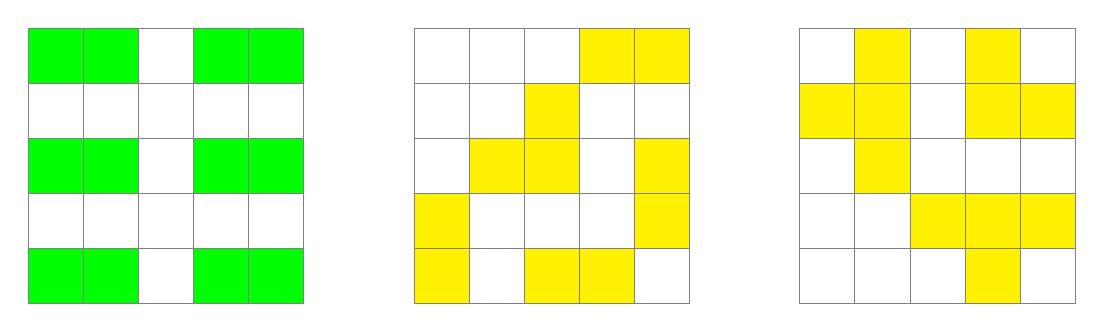
\begin{tikzpicture}[scale=0.7]
\path[fill=green] (0,0)--(0,1)--(2,1)--(2,0)--(0,0);
\path[fill=green] (0,2)--(0,3)--(2,3)--(2,2)--(0,2);
\path[fill=green] (0,4)--(0,5)--(2,5)--(2,4)--(0,4);
\path[fill=green] (3,0)--(3,1)--(5,1)--(5,0)--(3,0);
\path[fill=green] (3,2)--(3,3)--(5,3)--(5,2)--(3,2);
\path[fill=green] (3,4)--(3,5)--(5,5)--(5,4)--(3,4);
\draw[help lines] (0,0) grid (5,5);

\path[fill=yellow] (7,0)--(8,0)--(8,2)--(7,2)--(7,0);
\path[fill=yellow] (11,1)--(11,3)--(12,3)--(12,1)--(11,1);
\path[fill=yellow] (10,4)--(10,5)--(12,5)--(12,4)--(10,4);
\path[fill=yellow] (9,0)--(9,1)--(11,1)--(11,0)--(9,0);
\path[fill=yellow] (8,2)--(8,3)--(9,3)--(9,4)--(10,4)--(10,2)--(8,2);
\draw[help lines] (7,0) grid (12,5);

\path[fill=yellow] (14,3)--(14,4)--(15,4)--(15,5)--(16,5)--(16,2)--(15,2)--(15,3)--(14,3);
\path[fill=yellow] (17,3)--(19,3)--(19,4)--(18,4)--(18,5)--(17,5)--(17,3);
\path[fill=yellow] (16,1)--(16,2)--(19,2)--(19,1)--(18,1)--(18,0)--(17,0)--(17,1)--(16,1);
\draw[help lines] (14,0) grid (19,5);
\end{tikzpicture}
\end{center}
\end{sol}